\documentclass{report}
\usepackage[english]{babel}
\usepackage[bottom=4cm, top=3.5cm]{geometry}
\usepackage{fancyhdr}
\usepackage{graphicx}
\usepackage{float}
\usepackage[square,sort,comma,numbers]{natbib}
\usepackage{lipsum}

\usepackage{etoolbox}% http://ctan.org/pkg/etoolbox
\makeatletter
% \patchcmd{<cmd>}{<search>}{<replace>}{<success>}{<failure>}
% --- Patch \chapter
\patchcmd{\@makechapterhead}{50\p@}{\chapheadtopskip}{}{}% Space from top of page to CHAPTER X
\patchcmd{\@makechapterhead}{20\p@}{\chapheadsep}{}{}% Space between CHAPTER X and CHAPTER TITLE
\patchcmd{\@makechapterhead}{40\p@}{\chapheadbelowskip}{}{}% Space between CHAPTER TITLE and text
% --- Patch \chapter*
\patchcmd{\@makeschapterhead}{50\p@}{\chapheadtopskip}{}{}% Space from top of page to CHAPTER TITLE
\patchcmd{\@makeschapterhead}{40\p@}{\chapheadbelowskip}{}{}% SPace between CHAPTER TITLE and text
\makeatother
% Set new lengths
\newlength{\chapheadtopskip}\setlength{\chapheadtopskip}{10pt}
\newlength{\chapheadsep}\setlength{\chapheadsep}{30pt}
\newlength{\chapheadbelowskip}\setlength{\chapheadbelowskip}{15pt}

\renewcommand{\bibsection}{\chapter*{Literature}}

\begin{document}
\bibliographystyle{alphadin}

\begin{titlepage}
	\centering
	\includegraphics[width=0.15\textwidth]{example-image-1x1}\par 
	\vspace{1cm}
	{\scshape\LARGE University of Bern \\
	\large Computer Graphics Group\par}
	\vspace{1cm}
	{\scshape\Large Bachelor Thesis\par}
	\vspace{1.5cm}
	{\huge\bfseries Creation and modification of 3D meshes in virtual reality\par}
	\vspace{2cm}
	{\Large\itshape by Marcel Zauder\par}
	\vfill
	supervised by\par
	Prof. Dr. David \textsc{Bommes}
\end{titlepage}

\begin{abstract}
	Virtual Reality (VR) is one of the most up-and-coming technology sectors in informatics and already today a very important component in many different application areas. However, the search term ''virtual reality'' gives nearly 800'000'000 hits (as of March 2019). Also in the media VR covers more and more broadcasting time and therefore its acknowledgement is rapidly increasing.  Due to these many people nowadays know the term VR, but barely more than superficially and only a few of them have ever ventured into virtual reality. Even in modern companies, as architecture bureaus and the automobile industry, VR is used to create 3D models of prototypes so it can be shown to investors or to highlight problems or hints to make the product better. However, the biggest application of VR is in the gaming industry, in which this type of controlling is very well received. Therefore, it is not surprising that many companies are dealing with this area in order to further develop this technology. \\
	In this bachelor thesis a brief overview about VR is given and how it is used today. Especially highlighted is the usage of it in terms of the creation of 3D meshes. Considering this, already published programs from Google and Microsoft are inspected and their pros and cons are determined by executing a survey about intuitiveness and usability. Also the used Unreal Engine 4 and OpenVolumeMesh are introduced and presented. At the end of this bachelor thesis a completely new software for creating and modifying 3D meshes in VR is developed and proposed based on the specifications chosen during the process.
\end{abstract}

\tableofcontents

\chapter{Introduction}

\chapter{Research}

	\section{Virtual Reality}
		\subsection{Beginnings}
		\subsection{Today}
		\subsection{Future}
		
	\section{VR Hardware: HTC Vive}
	
	\section{Provided Software}
		In the following section a collection of 3D graphic software is presented and examined. In each of those applications it is possible to create 3D structures some rather on an architectural level some on an artistic level like drawing or modelling. Also the implementation of equal tools or the approach to the same task sometimes differ on a highly basis. \\
		Ideas and suggestions, which are drawn from these, then form the foundation of the program developed during the bachelor thesis.
		\subsection[Google Blocks]{Google Blocks \textsc{\small{\cite{GB4}}}}
			Google Blocks (latest version 4.0.10) is, compared to the other applications listed here, not a comprehensive but a very easy-to-use program. There are 6 main features at the moment: placement of ready-made 3D objects, drawing freehand lines, coloring, modifying, moving, and deleting objects and structures. Within these are also subfunctions, such as grouping, copying, and scaling up or down, available. The resulting scnenes can then be exported as .obj file or as an animated gif. There is also an own marketplace where creations of other users can be viewed and imported as well as own structures can be uploaded and published.
		\subsection[Google Tilt Brush]{Google Tilt Brush \textsc{\small{\cite{GTB}}}}
			Google Tilt Brush (latest version 18) offers the possibility to draw and paint in VR. Unlike the other softwares, here the artistic aspect and not the creation of volumetric meshes or 3D structures is at the point of interest. Therefore a work of art can be created with many different types of "dynamic brushes". A big variation provides the virtual palette which includes oil, ink, and water colors besides paints with effects as fire, glow, and smoke. Although it is possible to incorporate shapes into the scenery, this option is of less importance. \\
			For executing showcases to a group of observants in-game cameras can be placed, so creations can be viewed from different perspectives and not only in first-person.
		\subsection[Masterpiece VR]{Masterpiece VR \textsc{\small{\cite{MVR}}}}
			In Masterpiece VR (latest version 1.0.12.18.18.1) 3D  sculptures can be modelled by using "virtual clay". It is mainly used to create characters, objects, and asset visuals which then can be exported to Unity or Marmoset for example to be integrated in games. It is also possible to create very detailed objects due to the implementation of "pinch" and "noise" tools which roughen the surface of the clay sculptures. In addition the environment can be manipulated so each creation can be viewed under different light conditions and in various settings. \\
			Furthermore Masterpiece VR has the functionality to add collaborators and spectators to experience VR modelling in multiplayer.
		\subsection[Microsoft Maquette]{Microsoft Maquette \textsc{\small{\cite{MSM}}}}
			Microsoft Maquette (latest version 2019.1.0.0) 
			
	\section[Unreal Engine 4]{Unreal Engine 4 \textsc{\small{\cite{UE4}}}}	
		Unreal Engine 4 (UE4) is the latest version of the game engine developed by Epic Games. The first version of Unreal Engine appeared together with the FPS game Unreal in 1998 established by Tim Sweeney, the founder of said company. Due to be written in C++ and also being source-available since 2014 it can be implemented and imported very easily on many different platforms. By already supporting a huge amount of these platforms, it is a highly used engine for programming and setting up a multitude of various games. \\
		The framework consists of a graphic engine and its related script language UnrealScript among many other things. Also UnrealEd, a level editor, is provided with which the layout of maps and levels are changeable on the fly. With its possibility of blueprint visual scripting even complex prototypes can be intergrated in the virtual world without needing a high ackowledgement of coding. This makes Unreal Engine even suitable for the average programmer. By visualizing the different behaviours and dependencies the debugging is also quite easy. \\
		Because nowadays multiplayer experience is frequently used, adds even a scalable server/client architecture to get the ability to implement this component. Additionally, Unreal Engine has gathered a huge community behing itself which means that many different tools and feature integrations can already be downloaded and used via GitHub or the Marketplace. \\
		Through close collaboration between Epic Games and world's leading hardware and software manufacturers, UE4 is also geared towards the use of virtual reality (VR), augmented reality (AR), and mixed reality (MR) and therefore continues to evolve and improve in these areas.

	\section[OpenVolumeMesh]{OpenVolumeMesh \textsc{\small{\cite{OVM}}}}
		OpenVolumeMesh (OVM) is an open-source framework developed by M. Kremer, D. Bommes, and L. Kobbelt in 2013. It is a generic data structure based on OpenMesh to handle arbitrary polyhedral meshes. Therefore it uses the idea of half-edges and accordingly creates half-faces of different orientations. The biggest advantage of OVM, however, is that the data structure is equivalent to an indexed array, allowing access to run in constant time complexity. \\
		\begin{center}
			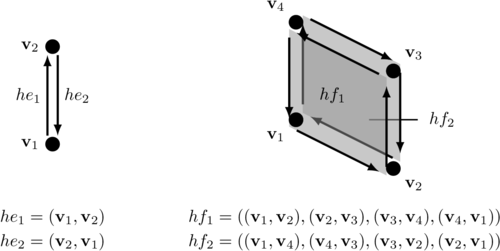
\includegraphics[width=0.5\textwidth]{halfedge_halfface.png} 
		\end{center}

\chapter{Intuition Study}

	\section{Concept and Execution}					
		To decide which specifications the new program should include and how they should be implemented, a test was performed in which two of the given programs, Google Blocks and Microsoft Maquette, were compared against each other and their intuitiveness was determined. Testworlds for Google Blocks as well as for Microsoft Maquette were created conducive to identify advantages and disadvantages of the individual features and to achieve the best possible implementation of the respective functionality. The tasks between these testing areas were kept as similar as possible so the measurement of the discrepancy of those two programs and their components is representative. In order to rule out that a program benefits by being tested secondarily, and thus previously learned could distort the test results, the process is always varied, so that half of the probands will start with Google Blocks and the other half with Microsoft Maquette. \\
		While the test persons are completing the tasks, notes are taken by the author wherein the intuitiveness of each service is checked according to how fast the functionality is discovered and understood as well as occuring problems are highlighted. At the end of this process an evaluation sheet, which contains questions about how intuitive and simple the different tasks were and which of the programs they preferred, is filled in.	

	\section{Tables}		
		In the following tables the results of the tests are listed. The scale for the movement part has been chosen differently (1-6), as it focuses on a more specific view to be able to study this functionality very closely and to determine what is perceived as a rather better type of movement. Concerning the other parts the point of interest was set on which program implemented each particular mode better. For illustrational purposes, the value of 1 has been assigned to the selected option. \\
		In the end the average value for each component was computed, so the usability and intuitiveness can be easily evaluated. \\			
		\begin{table}[H]
			\begin{tabular}{@{}|lll|llllllllllllll|r|@{}}
				\hline
				\multicolumn{3}{|l|}{\textbf{\underline{General}}} & & & & & & & & & & & & & & & \textbf{average $\emptyset$} \\ \hline
				& \multicolumn{2}{l|}{\textbf{Impression}} & & & & & & & & & & & & & & &\\ \hline
				& & Google Blocks & 1 & 0 & 1 & 1 & 1 & 1 & 0 & 1 & 0 & 1 & 1 & 0 & 0 & 0 & 0.57 \\
				& & Microsoft Maquette & 1 & 1 & 0 & 0 & 0 & 0 & 1 & 0 & 1 & 0 & 0 & 1 & 1 & 1 & 0.50 \\ \hline
				
				& \multicolumn{2}{l|}{\textbf{Simplicity}} & & & & & & & & & & & & & & &\\ \hline
				& & Google Blocks & 1 & 1 & 1 & 1 & 1 & 1 & 1 & 1 & 1 & 1 & 1 & 1 & 1 & 0 & 0.93 \\
				& & Microsoft Maquette & 0 & 0 & 0 & 1 & 0 & 0 & 0 & 0 & 0 & 0 & 0 & 0 & 0 & 1 & 0.13 \\ \hline
			\end{tabular}
			\caption{General Evaluation}
			\label{tab:tab3.1}
		\end{table}
		
		\begin{table}[H]			
			\begin{tabular}{@{}|lll|llllllllllllll|r|@{}}
				\hline
				\multicolumn{3}{|l|}{\textbf{\underline{Movement}}} & & & & & & & & & & & & & & & \textbf{average $\emptyset$} \\ \hline
				& \multicolumn{2}{l|}{\textbf{Intuitiveness}} & & & & & & & & & & & & & & &\\ \hline
				& & Google Blocks & 3 & 2 & 6 & 6 & 3 & 5 & 4 & 4 & 5 & 5 & 5 & 4 & 6 & 4 & 4.43 \\
				& & Microsoft Maquette & 3 & 2 & 5 & 4 & 2 & 4 & 4 & 2 & 4 & 1 & 3 & 5 & 5 & 3 & 3.36 \\ \hline
				
				& \multicolumn{2}{l|}{\textbf{Impression}} & & & & & & & & & & & & & & &\\ \hline
				& & Google Blocks & 4 & 1 & 6 & 5 & 6 & 5 & 3 & 5 & 5 & 5 & 5 & 4 & 5 & 4 & 4.50 \\
				& & Microsoft Maquette & 5 & 1 & 5 & 4 & 4 & 4 & 3 & 2 & 5 & 2 & 4 & 5 & 6 & 5 & 3.93 \\ \hline
			\end{tabular}	
			\caption{Movement Evaluation}
			\label{tab:tab3.2}	
		\end{table}
		\hfill \\
		\begin{table}[H]
			\begin{tabular}{@{}|lll|llllllllllllll|r|@{}}
				\hline
				\multicolumn{3}{|l|}{\textbf{\underline{Interface}}} & & & & & & & & & & & & & & & \textbf{average $\emptyset$} \\ \hline
				& & Google Blocks & 0 & 0 & 1 & 1 & 1 & 1 & 0 & 1 & 0 & 1 & 1 & 0 & 1 & 0 & 0.57 \\
				& & Microsoft Maquette & 1 & 1 & 0 & 0 & 0 & 0 & 1 & 0 & 1 & 0 & 1 & 1 & 1 & 1 & 0.57 \\ \hline
			\end{tabular}
			\caption{Interface Evaluation}
			\label{tab:tab3.3}
		\end{table}
		\hfill \\
		\begin{table}[H]
			\begin{tabular}{@{}|lll|llllllllllllll|r|@{}}
				\hline
				\multicolumn{3}{|l|}{\textbf{\underline{Object Interaction}}} & & & & & & & & & & & & & & & \textbf{average $\emptyset$} \\ \hline
				& \multicolumn{2}{l|}{\textbf{Placing}} & & & & & & & & & & & & & & &\\ \hline
				& & Google Blocks & 1 & 0 & 1 & 1 & 1 & 1 & 0 & 1 & 0 & 1 & 1 & 1 & 1 & 1 & 0.79 \\
				& & Microsoft Maquette & 1 & 1 & 0 & 1 & 0 & 0 & 1 & 0 & 1 & 0 & 0 & 0 & 0 & 0 & 0.36 \\ \hline
				
				& \multicolumn{2}{l|}{\textbf{Moving}} & \multicolumn{14}{c|}{\small{only Google Blocks implemented an explicit mode}} &\\ \hline
				& & Google Blocks & 1 & 0 & 1 & 1 & 1 & 1 & 1 & 1 & 1 & 1 & 1 & 0 & 1 & 1 & 0.86 \\
				& & Microsoft Maquette & 1 & 1 & 0 & 0 & 0 & 1 & 0 & 0 & 0 & 0 & 0 & 1 & 0 & 0 & 0.29 \\ \hline
				
				& \multicolumn{2}{l|}{\textbf{Snapping}} & & & & & & & & & & & & & & &\\ \hline
				& & Google Blocks & 0 & 0 & 1 & 1 & 1 & 1 & 1 & 1 & 1 & 1 & 1 & 1 & 0 & 0 & 0.71 \\
				& & Microsoft Maquette & 1 & 1 & 0 & 1& 0 & 0 & 0 & 0 & 0 & 0 & 0 & 1 & 1 & 1 & 0.43 \\ \hline
				
				& \multicolumn{2}{l|}{\textbf{Deleting}} & & & & & & & & & & & & & & &\\ \hline
				& & Google Blocks & 1 & 0 & 1 & 1 & 0 & 1 & 1 & 1 & 1 & 1 & 1 & 0 & 0 & 0 & 0.64 \\
				& & Microsoft Maquette & 1 & 1 & 0 & 1 & 1 & 0 & 1 & 0 & 1 & 0 & 1 & 1 & 1& 1 & 0.71\\ \hline
				
				& \multicolumn{2}{l|}{\textbf{Coloring}} & & & & & & & & & & & & & & &\\ \hline
				& & Google Blocks & 1 & 0 & 0 & 1 & 1 & 1 & 0 & 0 & 0 & 1 & 1 & 0 & 0 & 0 & 0.43 \\
				& & Microsoft Maquette & 0 & 1 & 1 & 1 & 1 & 0 & 1 & 1 & 1 & 0 & 0 & 1 & 1 & 1 & 0.71 \\ \hline
				
				& \multicolumn{2}{l|}{\textbf{Modifying}} & \multicolumn{14}{c|}{\small{only Google Blocks implemented an explicit mode}} &\\ \hline
				& & Google Blocks & 1 & 1 & 1 & 1 & 1 & 1 & 1 & 0 & 0 & 1 & 1 & 0 & 1 & 1 & 0.79\\
				& & Microsoft Maquette & 1 & 0 & 0 & 1 & 0 & 0 & 0 & 1 & 1 & 0 & 0 & 1 & 0 & 1 & 0.43 \\ \hline

				& \multicolumn{2}{l|}{\textbf{Grouping}} & \multicolumn{14}{c|}{\small{only Microsoft Maquette implemented an explicit mode}} &\\ \hline
				& & Google Blocks & 1 & 1 & 0 & 0 & 0 & 0& 1 & 1 & 1 & 0 & 0 & 1 & 0 & 0 & 0.43 \\
				& & Microsoft Maquette & 1 & 0 & 1 & 1 & 1 & 1 & 0 & 0 & 0 & 1 & 1 & 0 & 1 & 1 & 0.64 \\ \hline				
				
				& \multicolumn{2}{l|}{\textbf{Copying}} & \multicolumn{14}{c|}{\small{only Microsoft Maquette implemented an explicit mode}} &\\ \hline
				& & Google Blocks & 0 & 1 & 0 & 1 & 0 & 1 & 1 & 1 & 0 & 0 & 0 & 1 & 0 & 0 & 0.43 \\
				& & Microsoft Maquette & 1 & 0 & 1 & 1 & 1 & 0 & 1 & 0 & 1 & 1 & 1 & 0 & 1 & 1 & 0.71 \\ \hline
			\end{tabular}
			\caption{Object-Interaction Evaluation}
			\label{tab:tab3.4}					
		\end{table}
			
	\section{Results and Evaluation}
		\vspace{0.5cm}
		\subsection{Impression and Layout}
			In general neither program is significantly better or worse, nevertheless, a few discrepancies can be recognized between some functionalities. The main difference is within the simplicity, because Google Blocks has much fewer editing tools than Microsoft Maquette and is therefore considerably more surveyable and incomplex (referring Table \ref{tab:tab3.1}). \\
			Concerning the most interesting point, changing the in-game position, the survey shows, that Google Blocks is slightly easier to understand and to work with. However, moving through the world using the "swimming" concept of Maquette is not considered the best way to implement this essential part (referring Table \ref{tab:tab3.2}). A huge problem for both designs is that the "Grab" buttons, which are located on each side of both controllers, are difficult to use and not very handy. Therefore, these should only be used sporadically. \\
			In terms of the interface and selection menu none of these programs is especially better or worse than the other one (referring Table \ref{tab:tab3.3}). Nevertheless, it has been observed that the graphical display of the menu, which is located on the side of one controller, has often restricted and reduced the working area. To prevent this, it would be appropriate to implement a hiding option or place it so that it does not interfere with the user. A good example is Google Tilt Brush, where the selection menu is located above the controller. \\
		\subsection[Object Interaction]{Object Interaction \small{\texttt{(referring Table \ref{tab:tab3.4})}}}
			A general overview of the object interaction statistics suggests by implementing an explicit mode the associated tasks were perceived as much more pleasant and easier to use. This is also reflected in the fact that when one program had implemented a corresponding mode, whereas the other did not, that program was most likely to be considered more intuitive in that particular area. Therefore, this leads to the conclusion that for each interaction a demarcating mode should be implemented in order to ensure a high degree of user-friendliness. \\
			Placing given objects and shapes is quite similar in both tested programs, whereas generating freehand lines is much more easier in Microsoft Maquette because a more meaningful signifier is used. But in the study Google Blocks received a better rating. A reason for this is a much smaller, and therefore clearer, collection of given objects. Also switching between the different objects is easier in Google Blocks by swiping through using the touchpad. In Microsoft Maquette on the other hand every shape must be selected individually from the selection menu which is more inconvenient and time consuming. \\
			For moving objects Google Blocks implemented a specific "Grabbing"-mode so it was easier for the probands to figure out how to manipulate the position of structures. On the other hand Microsoft Maquette uses the "Grab"-buttons which intuitively makes sense because users are actually grabbing the thing. However, since the "Grab"-buttons are difficult to handle, the useability of this feature was considered rather bad. Therefore Google Blocks performed much better in that section and a significantly larger number of subjects considered it more pleasant. \\
			The applications include two different methods for implementing rotational snapping and alignment. In Google Blocks the left-handed trigger must be kept pressed, whereas in contrast Microsoft Maquette uses an additional button on the right-handed touchpad to toggle this mode on and off. The study found that the former was more comfortable to use, as the user did not need to check whether the mode is toggled on or off. \\
			There are two different variants for deleting objects in both softwares: On the one hand an independent mode is implemented, on the other hand, the object can be thrown away so it disappears. Especially the "Disposal"-option was considered very intuitive and useful. Since this feature is much more easily to apply and more reliable in Microsoft Maquette than Google Blocks, it was slightly better rated. \\
			Coloring in Google Blocks holds the problem in that the color palette is located on the back of the selection menu and is therefore not directly visible to the user. Consequently, a lot time was needed to find it, which ultimately had a negative impact on the user's opinion of this part. In Maquette the color selection was much more extensive, due to the implementation of an RGB palette. Also an eyedropper was added, whereby a color selection of already colored objects was possible. However, this involved the problem that the extraction line, which had to be directed onto the object to select the color, was not recognized as such, which made the handling of this option slightly difficult. Nonetheless, Microsoft Maquette did better in this area due to the greater color choice and the more convenient operation. \\
			Exclusively Google Blocks realized an explicit tool for modifying, as subdividing, extrude, and extract, objects and their assets, while in Microsoft Maquette only the length, width and depth of a structure are changeable. Also, handling the feature in Maquette, which requires a synchronized movement of both controllers, was not without problems. Accordingly, the test subjects perceived Google Blocks as a much more pleasent and better option for this type of interaction. \\
			For grouping and copying of several structures and objects both software have implemented an associated tool. In Google Blocks, however, this tool is hidden inside the "Grab" feature, which means it is not directly recognized. In contrast, in Microsoft Maquette, there are even several fields, within the copy function, into which object groups can be copied in order to quickly duplicate them. These details ultimately lead to Maquette performing better in the survey for both options, and more test subjects found it more easier to use. \\
		\subsection{Conclusion}
			The survey generally shows that each function is much more easier to use if there is a seperate, special mode for it. In addition, each of these modes should be clearly described and the functionality easy to recognize and quickly understood. Also, within a mode not many other specifications should be present, as this leads to a higher degree of complexity of the program. \\
			From the testers' reports and the author's notes, it further emerges that the "Grab"-buttons are very difficult to use, and thus an "over-use" of them is considered negative. On the other hand, the touchpad is acknowledged as a very good control option, so a good implementation of this can lead to a high level of usability. What is also noticeable is that many testers favor haptic feedback as very useful and should therefore be taken into account. \\
			Another problem was that the orientation of the interface menu often serverely restricted the workspace. Thus, an implementation as found in Google Tilt Brush with this menu above the secondary controller should be considered. Also a toggle mode to hide and show the menu can counteract this problem. \\
			Ultimately, this study has produced some ideas for implementing various specifications and has been able to inform about the differences in the usability of the modes. In Chapter 4 "Specifications" further details of the tools are analyzed.
	
\chapter{Specifications}
	The newly developed program, which will be the result of this bachelor thesis, contains the following specifications:
	\begin{description}
		\item placing single vertices
		\item placing edges \\
			whether the starting and the end point are predefined or dynamically created
		\item construct faces \\
			starting and end point must be the same to confirm \\
			possibility to add edges to a face
		\item "Snapping" mode \\
			\begin{itemize}
				\setlength{\itemsep}{0pt}
				\item[-] "on plain" (in the middle of a face etc.) \\
				\item[-] degree snapping (preset)
			\end{itemize}
	\end{description}
	-Einzelne Vertices setzen
	-Edges setzen
		-Anfangs- und Endpunkt sind schon gesetzt
		-Endpunkt wird gleichzeitig gesetzt
		-Anfangs- und Endpunkt werden selbst bestimmt
	Faces erstellen
		-Anfangs- und Endpunkt müssen der Gleiche sein, um zu bestätigen
		-Auswahl von Edges, um diese zu Face hinzuzufügen
	Snapping Modus
		-auf Fläche (mittig eines Faces etc.)
		-Grad (selber einstellbar??)
		-Länge? (noch nicht)
	
	Kamera aufstellen, um ein weiteres Fenster mit jenem Blickwinkel zu öffnen (für Showcases) (veränderbar)
	
	Färben (von Flächen [und Knoten für Farbübergänge?])
		-später Palette (nur wenige Farben)
	
	Showmodus
		-Hervorheben des Zeigebereichs
		
	Multiplayerfähig (per Default schon in UE4 integriert)
	
	Modifizierungsmodus
		-Extrude
		-Subdividing
		-Verschiebungsmodus von Vertices, Edges und Faces
	
	Fehler wird angezeigt (damit User diesen beheben kann)
		
	Objekt bewegen (dafür wird kein eigener Bewegungsmodus des Spielers benötigt, da normalerweise nur ein Objekt vorliegt)
		-eventuell Zoomeffekt?
		
	Zellen für OVM
		-Qualitätsmetriken
		
\chapter{Implementation}

\chapter{Documentation: OpenVolumeMeshVR}


\newpage
\addcontentsline{toc}{chapter}{Literature}
\bibliography{literature}
\end{document}
